% Provenance (never printed): cycle 3 "La planete Terre. Les etres vivants
% dans leur environnement" (natural phenomena: volcanoes and earthquakes,
% natural hazards and the behaviour to adopt); see sources/book1/PROVENANCE.md.
% Book 1, grade 4, chapter 2.
\chapter{火山与地震：初识}\label{ch:g4:volcanoes-earthquakes-first-look}

周一晚上，新闻播出了一座遥远岛屿上的\omterm{def:g4:volcanoes-earthquakes-first-look:volcano}{火山}。在
黑暗中，一股炽热的橙红色\omterm{def:g4:volcanoes-earthquakes-first-look:eruption}{熔岩}喷泉从地面的裂缝中喷涌而出，
火红的\omterm{def:g4:volcanoes-earthquakes-first-look:eruption}{熔岩}河缓缓流下山坡，流入大海，发出嘶嘶声，
冒着蒸汽。周四，新闻播出了另一个地方：一座小镇，
黎明时分，地面震动了半分钟。烟囱倒在街道上，
一座老房子从地基上滑落。

两件截然不同的事件。然而，它们都来自地球深处，
正如我们将看到的，它们在世界某些地区
发生的次数远多于其他地区。

\begin{recall}
山、\omterm{def:g1:landscapes-around-us:landform}{丘陵}、\omterm{def:g1:landscapes-around-us:landform}{山谷}和\omterm{def:g1:landscapes-around-us:landform}{平原}都是陆地的形态
（见\cref{ch:g1:landscapes-around-us}）。地球的陆地分为
七大洲，由五大洋环绕；太平洋是最大的
\omterm{def:g2:water-on-earth:ocean}{海洋}（见\cref{ch:g3:continents-and-oceans}）。
\end{recall}

\section{火山喷发}

脚下很深的地方，地球非常炽热。在某些地方，那里的\omterm{def:g3:stones-pebbles-sand:rock}{岩石}
热得已经熔化。这种熔融\omterm{def:g3:stones-pebbles-sand:rock}{岩石}比周围的固体\omterm{def:g3:stones-pebbles-sand:rock}{岩石}
更轻，因此会缓缓上升，就像水中的软木塞。一旦
找到通往地表的出口，\omterm{def:g4:volcanoes-earthquakes-first-look:volcano}{火山}便形成了。

\begin{definition}[火山]\label{def:g4:volcanoes-earthquakes-first-look:volcano}
\emph{火山}\index{火山}是指地球深处的熔融\omterm{def:g3:stones-pebbles-sand:rock}{岩石}
喷出地表的地方，以及熔融\omterm{def:g3:stones-pebbles-sand:rock}{岩石}在此
一层层堆积而成的\omterm{def:g1:landscapes-around-us:landform}{丘陵}或山峰。
\end{definition}

\begin{definition}[喷发、熔岩与火山灰]\label{def:g4:volcanoes-earthquakes-first-look:eruption}
\emph{喷发}\index{喷发}是指\omterm{def:g4:volcanoes-earthquakes-first-look:volcano}{火山}喷出
熔融\omterm{def:g3:stones-pebbles-sand:rock}{岩石}、\omterm{def:g4:volcanoes-earthquakes-first-look:volcano}{火山}灰和气体的过程。\emph{熔岩}\index{熔岩}是指
喷涌到地表的熔融\omterm{def:g3:stones-pebbles-sand:rock}{岩石}，它流动后冷却、凝固成新的\omterm{def:g3:stones-pebbles-sand:rock}{岩石}。
\emph{火山灰}\index{火山灰}由喷发时吹入空中的细小\omterm{def:g3:stones-pebbles-sand:rock}{岩石}
和玻璃碎屑组成，落下时像灰色的雪。
\end{definition}

\begin{omfigure}
\begin{tikzpicture}[font=\small]
  % ground and deep rock
  \fill[brown!30] (-5,-2.6) rectangle (5,0);
  % the volcano
  \fill[black!40] (-4.2,0) -- (-0.6,3.0) -- (0.6,3.0) -- (4.2,0) -- cycle;
  \fill[black!55] (-0.6,3.0) -- (-0.35,2.75) -- (0.35,2.75) -- (0.6,3.0) -- cycle;
  % layers inside the cone
  \foreach \k in {1,2,3}
    \draw[black!25] (-4.2+1.0*\k,0) -- (-0.6+0.05*\k,3.0-0.25*\k);
  % molten rock rising from deep below
  \fill[orange!80!red] (-0.25,-2.6) -- (-0.25,2.75) -- (0.25,2.75) -- (0.25,-2.6) -- cycle;
  \fill[orange!80!red] (0,-2.6) ellipse (1.6 and 0.5);
  % lava flow on the right flank
  \fill[orange!90!red] (0.5,2.9) .. controls (1.2,2.2) and (1.4,1.6) .. (2.2,1.0)
    .. controls (2.6,0.6) and (3.2,0.25) .. (3.7,0.1) -- (3.3,0.1)
    .. controls (2.6,0.35) and (2.0,0.75) .. (1.7,1.1)
    .. controls (1.2,1.6) and (0.9,2.3) .. (0.3,2.9) -- cycle;
  % ash and gas cloud
  \foreach \x/\y/\r in {0/3.6/0.45, -0.5/4.2/0.55, 0.4/4.3/0.5, -0.2/4.9/0.6, 0.6/5.0/0.55, -0.9/4.8/0.45, 0.1/5.5/0.6}
    \fill[black!25] (\x,\y) circle (\r);
  % labels
  \node[anchor=west] at (2.3,5.0) {火山灰和气体};
  \draw[black!60] (2.25,5.0) -- (1.1,4.9);
  \node[anchor=west] at (3.3,1.6) {熔岩流};
  \draw[black!60] (3.25,1.6) -- (2.1,1.1);
  \node[anchor=east] at (-3.0,2.0) {火山};
  \draw[black!60] (-2.95,2.0) -- (-1.9,1.5);
  \node[anchor=west, align=left] at (1.9,-1.4) {熔融岩石上升 \\来自地下深处};
  \draw[black!60] (1.85,-1.4) -- (0.3,-1.2);
\end{tikzpicture}

{\small 正在\omterm{def:g4:volcanoes-earthquakes-first-look:eruption}{喷发}的\omterm{def:g4:volcanoes-earthquakes-first-look:volcano}{火山}（示意图，未按比例绘制）。熔融\omterm{def:g3:stones-pebbles-sand:rock}{岩石}从
地下深处上升，从顶部喷出：它沿山坡流下形成\omterm{def:g4:volcanoes-earthquakes-first-look:eruption}{熔岩}，同时\omterm{def:g4:volcanoes-earthquakes-first-look:eruption}{火山灰}和
气体被喷上天空。每次\omterm{def:g4:volcanoes-earthquakes-first-look:eruption}{喷发}都会为山体添加一层新的
岩层。}
\label{fig:g4:volcanoes-earthquakes-first-look:volcano}
\end{omfigure}

并非所有\omterm{def:g4:volcanoes-earthquakes-first-look:eruption}{喷发}都一样。有些\omterm{def:g4:volcanoes-earthquakes-first-look:eruption}{喷发}中，\omterm{def:g4:volcanoes-earthquakes-first-look:eruption}{熔岩}流动性强：它
平静地汇成炽热的\omterm{def:g4:volcanoes-earthquakes-first-look:eruption}{熔岩}河，可以流淌数千米，有时一直
流到大海。另一些\omterm{def:g4:volcanoes-earthquakes-first-look:eruption}{喷发}中，熔融\omterm{def:g3:stones-pebbles-sand:rock}{岩石}黏稠且含有大量气体，像
一瓶摇晃过的汽水：喷出时会爆炸，形成巨大的
\omterm{def:g4:volcanoes-earthquakes-first-look:eruption}{火山灰}柱，高高升入天空。

\begin{omfigure}
\begin{minipage}[b]{0.56\linewidth}\centering
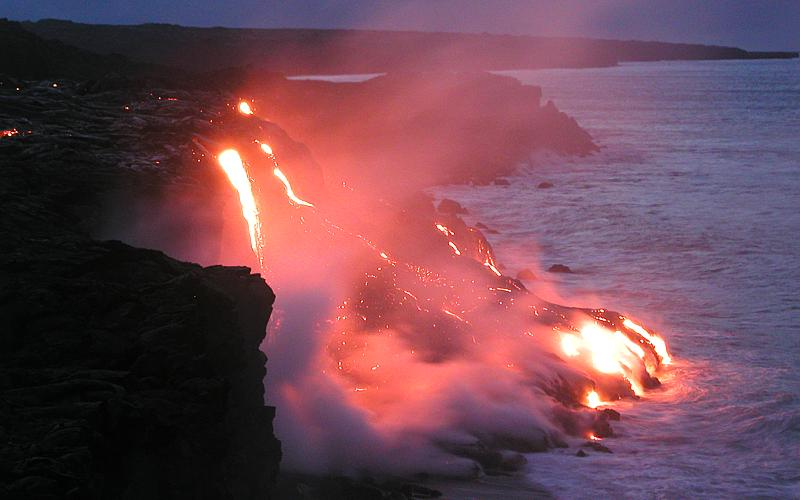
\includegraphics[width=\linewidth]{images/book1/g4-lava-ocean.jpg}

{\small 流动性强的\omterm{def:g4:volcanoes-earthquakes-first-look:eruption}{喷发}：\omterm{def:g4:volcanoes-earthquakes-first-look:eruption}{熔岩}从海边悬崖倾泻入海，地点在
夏威夷。照片：USGS Hawaiian Volcano Observatory（公有领域）。}
\end{minipage}\hfill
\begin{minipage}[b]{0.4\linewidth}\centering
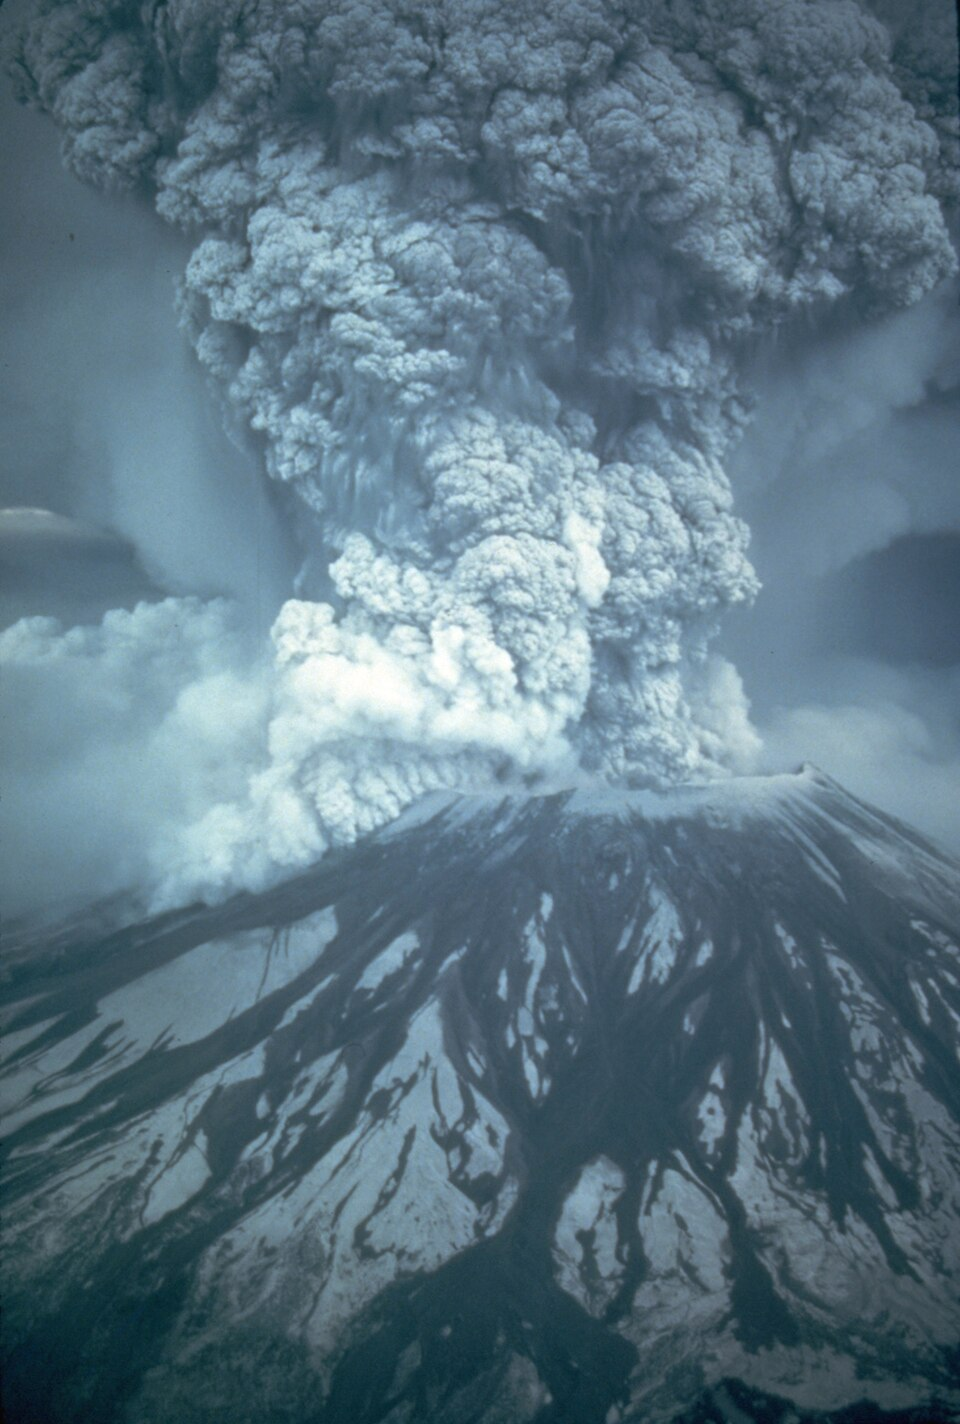
\includegraphics[width=0.78\linewidth]{images/book1/g4-st-helens.jpg}

{\small 爆炸式\omterm{def:g4:volcanoes-earthquakes-first-look:eruption}{喷发}：美国圣海伦斯\omterm{def:g4:volcanoes-earthquakes-first-look:volcano}{火山}，
1980 年 5 月 18 日。照片：Austin Post, USGS（公有领域）。}
\end{minipage}
% ledger: usgs:pu-oo-ocean, usgs:msh-1980
\label{fig:g4:volcanoes-earthquakes-first-look:two-eruptions}
\end{omfigure}

\begin{example}[圣海伦斯火山，1980 年]\label{ex:g4:volcanoes-earthquakes-first-look:st-helens}
1980 年春天，圣海伦斯\omterm{def:g4:volcanoes-earthquakes-first-look:volcano}{火山}一侧
出现了一处隆起，熔融\omterm{def:g3:stones-pebbles-sand:rock}{岩石}在山体内部向上推挤。5 月 18 日清晨，
一次小\omterm{def:g4:volcanoes-earthquakes-first-look:earthquake}{地震}震动了山体，隆起部分
在一场巨大的滑坡中滑落，\omterm{def:g4:volcanoes-earthquakes-first-look:volcano}{火山}向侧面和上方猛烈爆发。山体的
顶部 400 米消失了，山顶变成了一个巨大的\omterm{def:g4:volcanoes-earthquakes-first-look:volcano}{火山}口。
% ledger: usgs:msh-1980
\end{example}

\section{地面在震动}

我们脚下深处的\omterm{def:g3:stones-pebbles-sand:rock}{岩石}并非完全静止。它们非常缓慢地
被推挤和拉扯，微微弯曲，像被两端按压的尺子，
直到某一刻突然断裂、错动。这一冲击使周围
数千米范围内的地面都随之震动。

\begin{definition}[地震]\label{def:g4:volcanoes-earthquakes-first-look:earthquake}
\emph{地震}\index{地震}是指
深埋在地下的\omterm{def:g3:stones-pebbles-sand:rock}{岩石}破裂、错动而引起的地面突然震动。
\end{definition}

\omterm{def:g4:volcanoes-earthquakes-first-look:earthquake}{地震}通常只持续几秒钟，
最大的\omterm{def:g4:volcanoes-earthquakes-first-look:earthquake}{地震}有时可持续一两分钟。大多数\omterm{def:g4:volcanoes-earthquakes-first-look:earthquake}{地震}非常微弱，没有人能感觉到，
只有仪器才能探测到它们。强烈的\omterm{def:g4:volcanoes-earthquakes-first-look:earthquake}{地震}可以使地面像船甲板一样晃动，
使道路开裂，使墙壁和房屋倒塌。

\begin{omfigure}
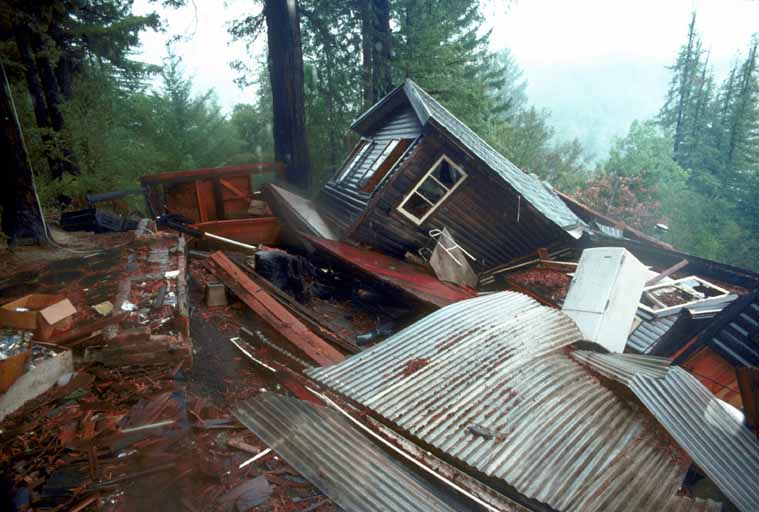
\includegraphics[width=0.55\linewidth]{images/book1/g4-loma-prieta-house.jpg}

{\small 1989 年加利福尼亚州发生强烈\omterm{def:g4:volcanoes-earthquakes-first-look:earthquake}{地震}后：这座木质房屋
被从混凝土地基上甩离原位。照片：J.~K.~Nakata，USGS
（公有领域）。}
% ledger: usgs:loma-prieta-house
\end{omfigure}

\begin{remark}[多久发生一次？]\label{rem:g4:volcanoes-earthquakes-first-look:how-often}
地质学家记录了地球上所有的大\omterm{def:g4:volcanoes-earthquakes-first-look:earthquake}{地震}。在 1976 年至 2025 年这 50 年间，
名单上共有 7\,031 次大\omterm{def:g4:volcanoes-earthquakes-first-look:earthquake}{地震}（强到足以损坏附近的建筑）：平均每年约 141 次，
即几乎每周 3 次。
能摧毁整座城镇的特大\omterm{def:g4:volcanoes-earthquakes-first-look:earthquake}{地震}，每年约 14 次。
地球上约有 1\,200 座\omterm{def:g4:volcanoes-earthquakes-first-look:volcano}{火山}在过去
约一万二千年里曾经\omterm{def:g4:volcanoes-earthquakes-first-look:eruption}{喷发}。
% ledger: data:usgs-comcat, data:gvp
\end{remark}

\section{火山与地震发生在哪里}

如果\omterm{def:g4:volcanoes-earthquakes-first-look:volcano}{火山}和\omterm{def:g4:volcanoes-earthquakes-first-look:earthquake}{地震}随机出现在任何地方，
\omterm{def:g3:continents-and-oceans:world-map}{世界地图}上的点就会均匀地散布在整张图上。事实并非如此。

下图显示了一个十分醒目的规律。大多数\omterm{def:g4:volcanoes-earthquakes-first-look:volcano}{火山}和大多数大\omterm{def:g4:volcanoes-earthquakes-first-look:earthquake}{地震}
都分布在狭长的带状区域中。其中最长的一条环绕太平洋：
从新西兰出发，向北经过印度尼西亚、菲律宾和
日本，横穿至阿拉斯加，然后沿美洲西\omterm{def:g1:landscapes-around-us:water}{海岸}一直向南，
直到智利南端。由于\omterm{def:g4:volcanoes-earthquakes-first-look:volcano}{火山}众多，它常被称为
“火环”。

\begin{example}[在地图上数一数]\label{ex:g4:volcanoes-earthquakes-first-look:shares}
我们数了落在阴影环带（距其中线 500~千米以内）的
点。在 1\,214 座\omterm{def:g4:volcanoes-earthquakes-first-look:volcano}{火山}中，837 座位于环带内，约每 3 座中有 2 座。
在 696 次特大\omterm{def:g4:volcanoes-earthquakes-first-look:earthquake}{地震}中，532 次位于环带内，约每 4 次中有 3 次。
环带只占地球的一小部分，
却集中了其中大部分的\omterm{def:g4:volcanoes-earthquakes-first-look:volcano}{火山}和\omterm{def:g4:volcanoes-earthquakes-first-look:earthquake}{地震}。
% ledger: data:gvp, data:usgs-comcat
\end{example}

\begin{omfigure}
\begin{tikzpicture}
\begin{axis}[ommap, width=\linewidth, xtick=\empty, ytick=\empty, grid=none,
    legend style={font=\scriptsize, at={(0.5,-0.02)}, anchor=north,
      draw=none, legend columns=3, /tikz/every even column/.append style={column sep=6pt}},
    legend cell align=left]
  \addplot[fill=omHypsLandA!85!black, draw=black!45, line width=0.2pt, forget plot]
    table {figdata/out/shared-geo-land.dat};
  \addplot[orange!80!black, opacity=0.35, line width=9pt, line cap=round, line join=round]
    table {figdata/out/grade-4-ring_of_fire-ring.dat};
  \addlegendentry{环绕太平洋的带状区域}
  \addplot[only marks, mark=triangle*, mark size=1.3pt, red!75!black]
    table[x=lon, y=lat] {figdata/out/grade-4-ring_of_fire-volcanoes.dat};
  \addlegendentry{火山（过去 12\,000 年内）}
  \addplot[only marks, mark=*, mark size=1.0pt, black, fill opacity=0.6]
    table[x=lon, y=lat] {figdata/out/grade-4-ring_of_fire-quakes7.dat};
  \addlegendentry{特大地震（1976--2025 年）}
\end{axis}
\end{tikzpicture}

{\small 过去约一万二千年内曾经\omterm{def:g4:volcanoes-earthquakes-first-look:eruption}{喷发}过的\omterm{def:g4:volcanoes-earthquakes-first-look:volcano}{火山}，以及
1976--2025 年间的特大\omterm{def:g4:volcanoes-earthquakes-first-look:earthquake}{地震}。它们大多沿着环绕太平洋的
一圈岛弧与山脉分布（阴影部分）。数据来源：
Smithsonian Global Volcanism Program；U.S. Geological
Survey earthquake catalogue；\omterm{def:g1:landscapes-around-us:water}{海岸}线：Natural Earth。}
\label{fig:g4:volcanoes-earthquakes-first-look:map}
% ledger: data:gvp, data:usgs-comcat, data:ne-land
\end{omfigure}

其他带状区域规模较小：一条横跨南欧和亚洲，
从地中海延伸到喜马拉雅山；另一些沿着大洋中部延伸，
那里的\omterm{def:g4:volcanoes-earthquakes-first-look:volcano}{火山}隐藏在海水之下。一些地方，比如
夏威夷，其\omterm{def:g4:volcanoes-earthquakes-first-look:volcano}{火山}远离任何带状区域。带状区域为何在这些位置，
这一问题将在\cref{ch:g7:plate-tectonics}中解答：答案解释了整张\omterm{def:g2:drawing-to-map:map}{地图}的格局。

\section{注意安全}

没有人能阻止\omterm{def:g4:volcanoes-earthquakes-first-look:volcano}{火山}\omterm{def:g4:volcanoes-earthquakes-first-look:eruption}{喷发}或\omterm{def:g4:volcanoes-earthquakes-first-look:earthquake}{地震}。但是，
知道该怎么做，就能挽救生命。

\begin{omfigure}
\begin{tikzpicture}[font=\small, line cap=round, line join=round]
  % --- panel 1: DROP onto hands and knees
  \begin{scope}
    \draw[black!30] (-0.2,0) -- (2.8,0);
    \fill[omDef] (0.62,0.98) circle (0.21);
    \draw[omDef, line width=2.2pt] (0.88,0.98) -- (2.0,0.95);
    \draw[omDef, line width=2pt] (0.95,0.96) -- (0.95,0.05);
    \draw[omDef, line width=2pt] (2.0,0.95) -- (1.98,0.08) -- (2.65,0.08);
    \node[font=\bfseries] at (1.3,-0.45) {趴下};
    \node[font=\scriptsize, align=center] at (1.3,-0.95) {双手和膝盖 \\着地};
  \end{scope}
  % --- panel 2: COVER under a table
  \begin{scope}[xshift=4cm]
    \draw[black!30] (-0.2,0) -- (2.8,0);
    \fill[brown!60!black] (-0.1,1.45) rectangle (2.7,1.6);
    \draw[brown!60!black, line width=2pt] (0.1,1.45) -- (0.1,0) (2.5,1.45) -- (2.5,0);
    \fill[omDef] (0.75,0.95) circle (0.2);
    \draw[omDef, line width=2.2pt] (0.95,0.85) -- (1.95,0.8);
    \draw[omDef, line width=2pt] (1.9,0.8) -- (1.65,0.05) -- (2.25,0.05);
    \draw[omDef, line width=2pt] (1.0,0.85) -- (0.7,1.2) -- (0.5,0.95);
    \node[font=\bfseries] at (1.3,-0.45) {掩护};
    \node[font=\scriptsize, align=center] at (1.3,-0.95) {保护头和颈部，\\躲到结实的桌子下};
  \end{scope}
  % --- panel 3: HOLD ON to the table leg
  \begin{scope}[xshift=8cm]
    \draw[black!30] (-0.2,0) -- (2.8,0);
    \fill[brown!60!black] (-0.1,1.45) rectangle (2.7,1.6);
    \draw[brown!60!black, line width=2pt] (0.1,1.45) -- (0.1,0) (2.5,1.45) -- (2.5,0);
    \fill[omDef] (0.75,0.95) circle (0.2);
    \draw[omDef, line width=2.2pt] (0.95,0.85) -- (1.95,0.8);
    \draw[omDef, line width=2pt] (1.9,0.8) -- (1.65,0.05) -- (2.25,0.05);
    \draw[omDef, line width=2pt] (1.0,0.85) -- (0.7,1.2) -- (0.5,0.95);
    \draw[omDef, line width=2pt] (1.0,0.8) -- (0.45,0.6) -- (0.12,0.65);
    \node[font=\bfseries] at (1.3,-0.45) {抓牢};
    \node[font=\scriptsize, align=center] at (1.3,-0.95) {抓住桌子，直到 \\震动停止};
  \end{scope}
\end{tikzpicture}

{\small 地面开始晃动时该怎么做：趴下、
掩护、抓牢。}
\label{fig:g4:volcanoes-earthquakes-first-look:drop-cover}
% ledger: shakeout:dch
\end{omfigure}

\begin{safety}
\textbf{\omterm{def:g4:volcanoes-earthquakes-first-look:earthquake}{地震}发生时。}一旦感觉到地面晃动：
\textbf{趴下}，双手和膝盖着地；用手臂\textbf{掩护}头部和脖子，
如果附近有结实的桌子或书桌，就爬到其下方；
\textbf{抓牢}桌子，直到震动停止。晃动时不要跑到室外，
也不要站在门口：坠落的玻璃和物体
是最主要的危险。停止后，要冷静地离开建筑物，
就像你在学校的演练中练习过的那样。

\textbf{靠近\omterm{def:g4:volcanoes-earthquakes-first-look:volcano}{火山}。}科学家监测可能苏醒的\omterm{def:g4:volcanoes-earthquakes-first-look:volcano}{火山}。若
他们预警即将\omterm{def:g4:volcanoes-earthquakes-first-look:eruption}{喷发}，有关部门会通知人们
撤离该地区。请立即听从他们的指示，切勿前往靠近观看。
\end{safety}
% ledger: shakeout:dch

\begin{omfigure}

\includegraphics[width=0.55\linewidth]{images/book1/ai/g4-earthquake-drill.jpg}

{\small \omterm{def:g4:volcanoes-earthquakes-first-look:earthquake}{地震}演练：学生们在课桌下练习“趴下、掩护、
抓牢”。}
\end{omfigure}

\section{练习}

\begin{exercise}[$\star$]\label{exo:g4:volcanoes-earthquakes-first-look:1}
\omterm{def:g4:volcanoes-earthquakes-first-look:eruption}{熔岩}、\omterm{def:g4:volcanoes-earthquakes-first-look:eruption}{火山灰}还是气体？(a) 沿斜坡流下、发着光的炽热\omterm{def:g4:volcanoes-earthquakes-first-look:eruption}{熔岩}流；
(b) 被喷到空中、又像灰色雪花一样落下的细小\omterm{def:g3:stones-pebbles-sand:rock}{岩石}碎片；
(c) 随\omterm{def:g4:volcanoes-earthquakes-first-look:eruption}{火山灰}一起从\omterm{def:g4:volcanoes-earthquakes-first-look:volcano}{火山}中逸出的、看不见的物质。
\end{exercise}

\begin{exercise}[$\star$]\label{exo:g4:volcanoes-earthquakes-first-look:2}
什么是\omterm{def:g4:volcanoes-earthquakes-first-look:earthquake}{地震}？它持续的是几小时，还是几秒钟？
\end{exercise}

\begin{exercise}[$\star$]\label{exo:g4:volcanoes-earthquakes-first-look:3}
将三个步骤按正确顺序排列：抓牢；趴下；掩护。
\end{exercise}

\begin{exercise}[$\star$]\label{exo:g4:volcanoes-earthquakes-first-look:4}
在第~\pageref{fig:g4:volcanoes-earthquakes-first-look:map}~页的\omterm{def:g2:drawing-to-map:map}{地图}上，大多数\omterm{def:g4:volcanoes-earthquakes-first-look:volcano}{火山}
围绕哪一个\omterm{def:g2:water-on-earth:ocean}{海洋}分布？
\end{exercise}

\begin{exercise}[$\star$]\label{exo:g4:volcanoes-earthquakes-first-look:5}
判断对错：(a) 大多数\omterm{def:g4:volcanoes-earthquakes-first-look:earthquake}{地震}都太小，人感觉不到；(b) \omterm{def:g4:volcanoes-earthquakes-first-look:eruption}{熔岩}
会永远保持液态；(c) 地面晃动时，最安全的做法是
跑到室外。
\end{exercise}

\begin{exercise}[$\star$]\label{exo:g4:volcanoes-earthquakes-first-look:6}
观察第~\pageref{fig:g4:volcanoes-earthquakes-first-look:volcano}~页上的\omterm{def:g4:volcanoes-earthquakes-first-look:volcano}{火山}示意图。
岩浆从哪里来？又从哪里喷出？
\end{exercise}

\begin{exercise}[$\star\star$]\label{exo:g4:volcanoes-earthquakes-first-look:7}
在\omterm{def:g2:drawing-to-map:map}{地图}上找出：(a) 美洲的一个国家，其全境沿线分布着许多\omterm{def:g4:volcanoes-earthquakes-first-look:volcano}{火山}；
(b) 太平洋中部的一组岛屿，上面有\omterm{def:g4:volcanoes-earthquakes-first-look:volcano}{火山}，
但不在环带上。
\end{exercise}

\begin{exercise}[$\star\star$]\label{exo:g4:volcanoes-earthquakes-first-look:8}
每年大约发生 141 次大\omterm{def:g4:volcanoes-earthquakes-first-look:earthquake}{地震}。平均每个
月大约有多少次？（一年有 12 个月；请给出整数。）
\end{exercise}

\begin{exercise}[$\star\star$]\label{exo:g4:volcanoes-earthquakes-first-look:9}
大约每 4 次特大\omterm{def:g4:volcanoes-earthquakes-first-look:earthquake}{地震}中就有 3 次发生在环绕太平洋的
\omterm{def:g4:volcanoes-earthquakes-first-look:earthquake}{地震}带上。若有 20 次特大\omterm{def:g4:volcanoes-earthquakes-first-look:earthquake}{地震}，你估计其中大约有多少次
发生在该\omterm{def:g4:volcanoes-earthquakes-first-look:earthquake}{地震}带上？又有多少次在该带之外？
\end{exercise}

\begin{exercise}[$\star\star$]\label{exo:g4:volcanoes-earthquakes-first-look:10}
在一次\omterm{def:g4:volcanoes-earthquakes-first-look:earthquake}{地震}演练中，利奥跑到教室门口站着。他
本应怎样做？为什么？
\end{exercise}

\begin{exercise}[$\star\star\star$]\label{exo:g4:volcanoes-earthquakes-first-look:11}
\omterm{def:g2:drawing-to-map:map}{地图}上共有 1\,214 座\omterm{def:g4:volcanoes-earthquakes-first-look:volcano}{火山}，其中 837 座位于环绕太平洋的
\omterm{def:g4:volcanoes-earthquakes-first-look:volcano}{火山}带上。环带之外有多少座？用“大约三分之二”
来描述环带内的占比是否恰当？（提示：1\,200 的三分之二是多少？）
\end{exercise}
